\documentclass[aspectratio=169, 12pt]{beamer}
\usepackage{amsmath,amssymb,amsfonts}
\usepackage{ctex}
\usepackage{graphics}
\usepackage[url = false, doi = false, backend=biber,style=gb7714-2015,gbalign=gb7714-2015,gbpub=false,gbmedium=false]{biblatex}
\usepackage{subfigure}
\usepackage{xcolor}
\usepackage{minted}
\colorlet{shadecolor}{gray!15}
\usefonttheme[onlymath]{serif}
\setbeamertemplate{caption}[numbered]
\usetheme{CambridgeUS}  
\usecolortheme{dolphin}  
\setcounter{tocdepth}{2}
\graphicspath{{../figures/}}
\addbibresource{../ref.bib}
\title{利用Qutip研究拉比振荡}
\author[周子正.等]{周子正\ 朱哲昊\ 孙蔚轩}
\institute[南开大学]{南开大学\ 物理科学学院、金融学院}
\date{\today}

\begin{document}
\begin{frame}
    \titlepage
    \centering
    \small 项目地址:
    \url{https://github.com/NKUPythonLessonProject/Rabi-Oscillation}
\end{frame}
\AtBeginSection[]{\frame{\sectionpage}}
\begin{frame}
    \tableofcontents[hideallsubsections]
\end{frame}

\section{理论分析}

\begin{frame}
    \frametitle{背景}
    对二能级系统,施加频率恰当电磁波,系统中的原子会不断在能级间跃迁,称之为拉比振荡\cite{zhu_vacuum_1990}。

    \vspace{.7cm}

    拉比振荡广泛应用于量子计算、量子光学和凝聚态物理等领域。拉比震荡至今仍然有广泛的研究。

    \vspace{.7cm}

    2020年,南开大学物理科学学院陈志刚教授、许京军教授领导的课题组理论研究发现,手性存在于拉比振荡的相位演化中\cite{zhang_unveiling_2020}。
\end{frame}

\begin{frame}
    \frametitle{Hamiltonian}
    根据Jaynes - Fred Cummings 模型\cite{jaynes_comparison_1963}\cite{cummings_reminiscing_2013},在谐振器内的二能级原子体系的哈密顿量可以构造为:
    \begin{equation}
        \hat{H}=\hbar \omega \hat{a}^{\dagger} \hat{a}+\hbar \omega_{0} \frac{\hat{\sigma}_{z}}{2}+\hbar g\left(\hat{a} +\hat{a}^{\dagger} \right)\left(\hat{\sigma}_{-}+\hat{\sigma}_{+}\right).
        \label{equ:H}
    \end{equation}

    $\hbar\omega$是光量子能量、$\hbar\omega_0$是原子内部能级的能隙。$g$是耦合强度。当取$\delta  = \omega-\omega_0$趋于0时,体系的振动频率为$\Omega_r = 2g$,这就是拉比振荡的频率。
\end{frame}

\begin{frame}[shrink]
    \frametitle{四种可能过程}
    \begin{columns}[t]

        \column{0.3\linewidth}

        我们已经构造了完整的Hamiltonian,如Eq. \ref{equ:H}。类比费曼图,可以画出其中发生的四个过程,如图\ref{fig:4-process}。

        图\ref{fig:4-process}中$\hat{a}^\dagger\sigma_+$和$\hat{a} \sigma_-$项的贡献在慢变场情况可以忽略。

        \column{0.7\linewidth}

        \begin{figure}
            \centering
            \subfigure[]{
                \centering
                \begin{minipage}[t]{0.45\textwidth}
                    \centering
                    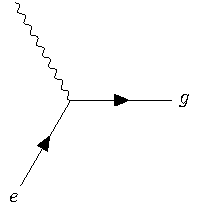
\includegraphics[height=2cm,width=2cm]{fig1.pdf}
                \end{minipage}%
                \begin{minipage}[t]{0.45\textwidth}
                    \centering
                    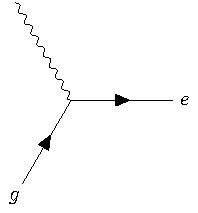
\includegraphics[height=2cm,width=2cm]{fig2.pdf}
                \end{minipage}
            }\\
            \subfigure[]{
                \centering
                \begin{minipage}[t]{0.45\textwidth}
                    \centering
                    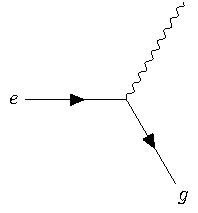
\includegraphics[height=2cm,width=2cm]{fig3.pdf}
                \end{minipage}%
                \begin{minipage}[t]{0.45\textwidth}
                    \centering
                    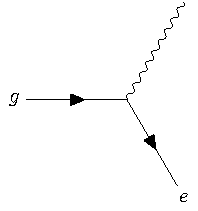
\includegraphics[height=2cm,width=2cm]{fig4.pdf}
                \end{minipage}
            }%
            \caption{四种可能过程}
            \label{fig:4-process}
        \end{figure}

    \end{columns}
\end{frame}

\begin{frame}
    \frametitle{旋转波近似}
    \begin{equation}
        \hat{H}=\hbar \omega \hat{a}^{\dagger} \hat{a}+\hbar \omega_{0} \frac{\hat{\sigma}_{z}}{2}+\hbar g\left(\hat{a} +\hat{a}^{\dagger} \right)\left(\hat{\sigma}_{-}+\hat{\sigma}_{+}\right).
    \end{equation}

    变为:

    \begin{equation}
        \hat{H}_{RWA}=\hbar \omega \hat{a}^{\dagger} \hat{a}+\hbar \omega_{0} \frac{\hat{\sigma}_{z}}{2}+\hbar g\left(\hat{a}\hat{\sigma}_{+} +\hat{a}^{\dagger}\hat{\sigma}_{-} \right),
        \label{equ:H-RWA}
    \end{equation}

    这个结果和旋转波近似\cite{wu_strong-coupling_2007}相同。

\end{frame}

\section{传统计算方法}
\begin{frame}[shrink]
    \frametitle{传统计算方法}
    在研究具体系统与实验的对应时,传统的求解方法是要将初态$\left|\psi(0)\right> = C_g(0)\left|g\right> + C_e(0)\left|e\right>$将外场的形式带入薛定谔方程直接计算或者处理成微扰项进行近似计算。

    在外场对时间只有平庸依赖$E = E_0 \exp(i\omega t)$的情况下可以写出其方程为:
    \begin{equation}
        \begin{aligned}
            \frac{d}{d t} C_{e} & =-i \frac{\omega_{0}-\omega}{2} C_{e}-i \Omega_{r} C_{g} \\
            \frac{d}{d t} C_{g} & =+i \frac{\omega_{0}-\omega}{2} C_{g}-i \Omega_{r} C_{e}
        \end{aligned}
    \end{equation}

    若同时$\Omega_r$与时间无关时,此方程可以精确求解。其振动频率为$\Omega_r$。对于更加一般的问题,由于不能精确求解方程,处理方法是利用数值方法进行求解。

\end{frame}
\section{Qutip计算方法}
\begin{frame}
    \frametitle{Qutip简介}
    Python中的Quantum Toolbox(QuTiP)是一个用Python编程语言编写的开源框架\cite{johansson_qutip_2012}\cite{johansson_qutip_2013},旨在模拟上述系统的开放量子动力学。
    QuTiP是一个开源软件,可以随意修改和使用。它基于Python脚本语言,易于阅读,可以快速生成代码,无需修改后再进行编译。QuTiP旨在提供各种用户友好的和高效的哈密顿量的数值模拟,包括具有任意时间依赖性的哈密顿量,还能与Matplotlib包和Numpy包交互。

\end{frame}

\begin{frame}[fragile,shrink]
    \frametitle{利用Qutip构建系统的哈密顿量}
    Qubit对无限维的光子场无法处理,在研究问题的背景下,其希尔伯特空间可以通过截断进行处理,此时可以定义出其哈密顿量为:
    \begin{minted}[fontsize=\footnotesize,frame=lines,python3,mathescape,bgcolor=shadecolor]{python}
        N = 50
        #$\hat a$
        a = tensor(destroy(N), qeye(2))
        #$\hat \sigma$
        sm = tensor(qeye(N), destroy(2))
        #$\hat H$
        H = wc * a.dag() * a + wa * sm.dag() * sm \
        + 0.5 * wr * (a.dag() * sm + a * sm.dag())
    \end{minted}
\end{frame}

\begin{frame}[fragile]
    \frametitle{初态定义为}
    \begin{minted}[fontsize=\footnotesize,frame=lines,python3,mathescape,bgcolor=shadecolor]{python}
        #$\left|\psi(0)\right>$
        psi0 = tensor(basis(N, n), cg * basis(2, 0) \
            + ce * basis(2, 1))
    \end{minted}
    态随时间演化可以利用$mesolve$求出。特别的,实践中一般关注特定算符的期望值,算符的期望值随时间的演化可以直接求出。

    振荡的形式类似于三角函数,通过拟合可以求出其振荡频率。使用scipy包的optimize.curve\_fit方法拟合,可以得到振荡频率与参数相符,证明模拟是正确的。
\end{frame}

\begin{frame}
    \frametitle{频率条件}
    \begin{columns}
    \column{0.4\linewidth}
    当失谐$\delta = \omega_0 - \omega$不趋近于0时,拉比振荡不会发生,此情况结果为图\ref{fig:1}所示。
    \column{0.6\linewidth}
    \begin{figure}
        \centering
        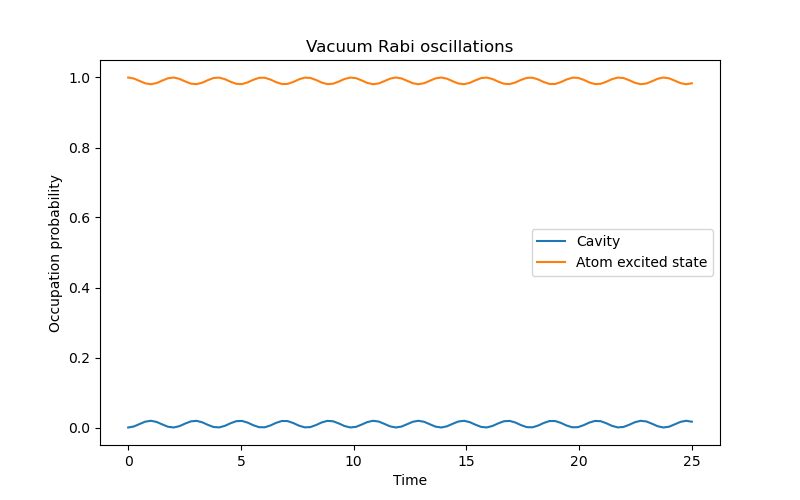
\includegraphics[width=0.8\linewidth]{1.png}
        \caption{振荡频率条件破坏}
        \label{fig:1}
    \end{figure}
    \end{columns}
\end{frame}

\begin{frame}[fragile]
    \frametitle{求解方法}
    \begin{minted}[fontsize=\footnotesize,frame=lines,python3,mathescape,bgcolor=shadecolor]{python}
        wc = 1.0 * 2 * np.pi
        wa = 1.5 * 2 * np.pi
        wr = 0.05 * 2 * np.pi
        H = Get_H_operator(wc, wa, wr, True)
        psi0 = Get_initial_state(0, 1, 0)
        tlist = np.linspace(0, 25, 100)
        c_op_list = Get_c_ops(0, 0, 0)
        output = mesolve(H, psi0, tlist, c_op_list,\
         [a.dag() * a, sm.dag() * sm])
    \end{minted}
\end{frame}

\begin{frame}
    \frametitle{能量传递}
    \begin{columns}
    \column{0.2\linewidth}
    当失谐取0时,可以对拉比振荡进行求解,作为一个示例,取初态原子全部处于激发态,光场不携带能量。
    \column{0.4\linewidth}
    \begin{figure}
        \centering
        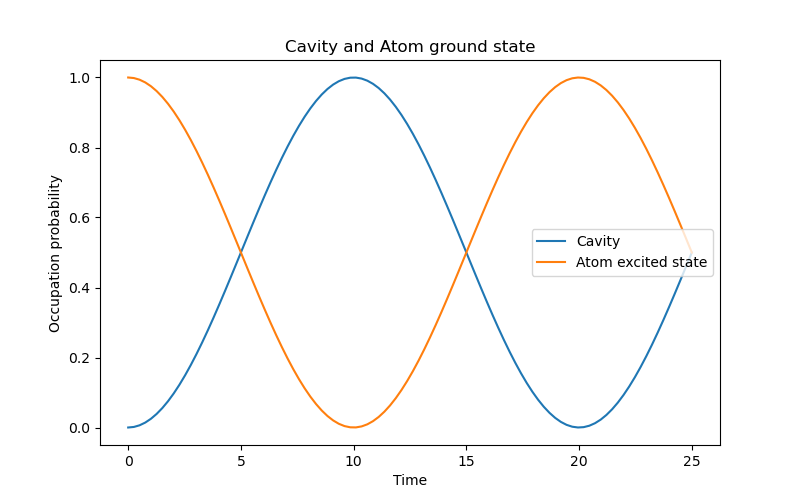
\includegraphics[width=1.0\linewidth]{3.png}
        \caption{光场和原子之间的能量转移}
        \label{fig:3}
    \end{figure}
    \column{0.4\linewidth}
    \begin{figure}
        \centering
        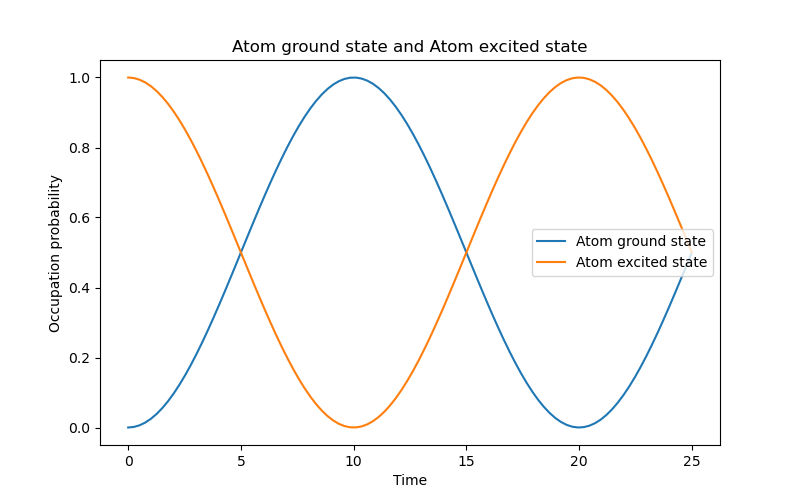
\includegraphics[width=1.0\linewidth]{2.png}
        \caption{基态和激发态之间的能量传递}
        \label{fig:2}
    \end{figure}
    \end{columns}
\end{frame}

\begin{frame}
    \frametitle{RWA近似失效}
    \begin{columns}
    \column{0.2\linewidth}
    旋转波近似实际上只适用于低频情况,通过图\ref{fig:3}、\ref{fig:4}对比可以看到,在高频条件下旋转波近似的结果与实际结果偏离很大。
    \column{0.4\linewidth}
    \begin{figure}
        \centering
        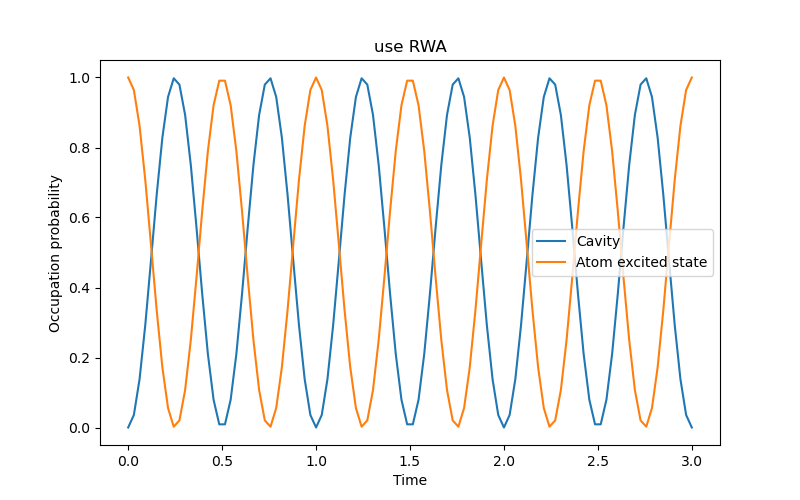
\includegraphics[width=1.0\linewidth]{4.png}
        \caption{RWA近似}
        \label{fig:4}
    \end{figure}
    \column{0.4\linewidth}
    \begin{figure}
        \centering
        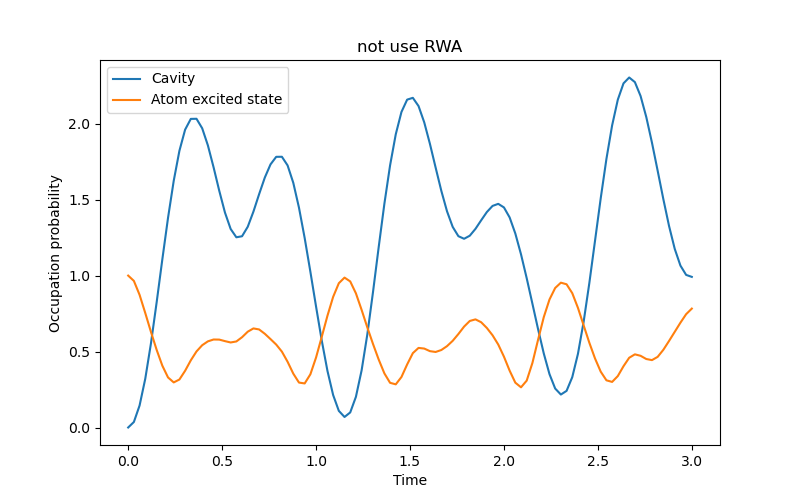
\includegraphics[width=1.0\linewidth]{5.png}
        \caption{实际情况}
        \label{fig:5}
    \end{figure}
    \end{columns}
\end{frame}

\begin{frame}
    \frametitle{耗散效应}
    \begin{columns}
    \column{0.4\linewidth}
    实际实验中包含了各种情况的耗散,耗散也可以利用Qutip框架进行计算。
    \column{0.6\linewidth}
    \begin{figure}
        \centering
        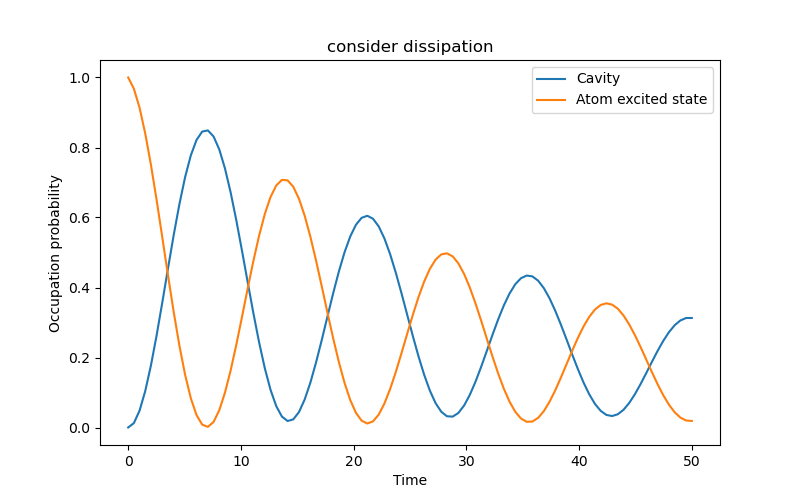
\includegraphics[width=0.8\linewidth]{6.png}
        \caption{能量耗散}
        \label{fig:6}
    \end{figure}
    \end{columns}
\end{frame}

\section{结论}
\begin{frame}
    \frametitle{结论}
    拉比振荡的传统计算方法是采用数值法求解微分方程。本文使用python语言,利用Qutip框架,根据Jaynes - Fred Cummings 模型,计算了拉比振荡过程中算符本征值随时间的演化。

    我们验证了拉比振荡的频率条件,RWA近似的使用范围,对拉比振荡进行了模拟与可视化,通过数据分析方法验证了拉比振荡的频率结果。
\end{frame}

\section{参考文献}
\begin{frame}[allowframebreaks]
    \frametitle{参考文献}
    \printbibliography[heading=none]
\end{frame}

\end{document}